\documentclass{aircc}
\usepackage{mathpartir}
\usepackage{listings}
\usepackage{booktabs}
\usepackage{graphicx}
\usepackage{graphics}
\usepackage{geometry}
\usepackage{listings}
\usepackage{xcolor}
\usepackage{anyfontsize}

\definecolor{codegreen}{rgb}{0,0.6,0}
\definecolor{codegray}{rgb}{0.5,0.5,0.5}
\definecolor{codepurple}{rgb}{0.58,0,0.82}
\definecolor{backcolour}{rgb}{0.95,0.95,0.92}

\lstdefinestyle{mystyle}{
    backgroundcolor=\color{backcolour},   
    commentstyle=\color{codegreen},
    keywordstyle=\color{magenta},
    numberstyle=\color{codegray},
    stringstyle=\color{codepurple},
    basicstyle=\ttfamily\footnotesize,
    breakatwhitespace=false,         
    breaklines=true,                 
    captionpos=b,                    
    keepspaces=true,                 
    numbers=left,                    
    numbersep=5pt,                  
    showspaces=false,                
    showstringspaces=false,
    showtabs=false,                  
    tabsize=2
}
\lstset{style=mystyle}

\begin{document}

\title{What's in a Domain? Analysis of URL Features}

\author{John Hawkins}
\affiliation{Transitional AI Research Group\\Getting-Data-Science-Done.com}

\maketitle

\begin{abstract}
Many data science problems require processing log data derived from web pages, APIs or other
internet traffic sources. URLs are one of the few ubiquitous data fields that describe
internet activity, hence they require effective processing for a wide variety of machine 
learning applications. While URLs are structurally rich, the structure can be both domain 
specific and subject to change over time, making feature engineering for URLs an ongoing 
challenge.

In this research we outline the key structural components of URLs and discuss the information
available within each. We describe methods for generating features on these URL components and 
share an open source implementation of these ideas. In addition, we describe a method for 
exploring URL feature importance that allows for comparison and analysis of the information 
available inside URLs.
We experiment with a collection of URL classification datasets and demonstrate the utility 
of these tools. Package and source code is open on \textit{https://pypi.org/project/url2features}
\end{abstract}

\begin{keywords}
Machine Learning, Feature Engineering, Web Search, Semantic Web, Data Science
\end{keywords}

\section{Introduction}

The Uniform Resource Locator (URL) is a ubiquitous element in the digital world. 
We use them to retrieve news and media, advertise or find businesses and services, 
and to interact with other people across a broad range of social applications. Below the
surface many online services use URLs internally for communicating with other digital
services, making the URL a fundamental data point for both users and machines.

Processing URLs is a key component of many tasks that involve
analysing internet data. In many applications the URL is the central piece of 
information available because the demands of the task require immediate analysis.
In applications like malicious wesite detection the URL needs to be processed
in a rapid and efficient manner to provide utility\cite{Ma2009b}.
Common use cases for URL centered analysis include security analysis of potential 
phishing attacks\cite{Garera2007,Basnet2012,Basnet2014,Mamun2016,Verma2017,Vazhayil2018,Tupsamudre2019,Sirigineedi2020,Li2020}, 
and identification of pages that host malware or viruses \cite{Canali2011,Mamun2016}.
There are also applications to online advertising,
including anticipation of conversions \cite{Qiu2020}, contextual analysis of
the content\cite{Kan2004,Shih2004,Baykan2009,Meshkizadeh2010,Hernandez2012,Arya2016}, relevance \cite{Kan2005} 
or language\cite{Baykan2013} of webpages. 
Content categorisation has also been applied to spam web pages using URLs alone for the sake
of search results filtering\cite{Chung2010,Hassan2008}.

The URL is made up of multiple elements, but at its core is the domain. The domain
contains internal information about both the intended purpose of a URL, its legitimacy 
and the likely country of origin. The domain is also a source of additional information 
through requests to Domain Name Servers (DNS) to understand both its history and the
structure of its network topology and resources.

Beyond the domain, the URL consists of a sequence of words, categories, identifiers, dates
or domain specific abreviations. This sequence can indicate the psychological elements of how
information is categeoried, or the internal logic of an application that generates or presents
content dynamically. 

\begin{figure*}
\centering
\resizebox{\columnwidth}{!}{%
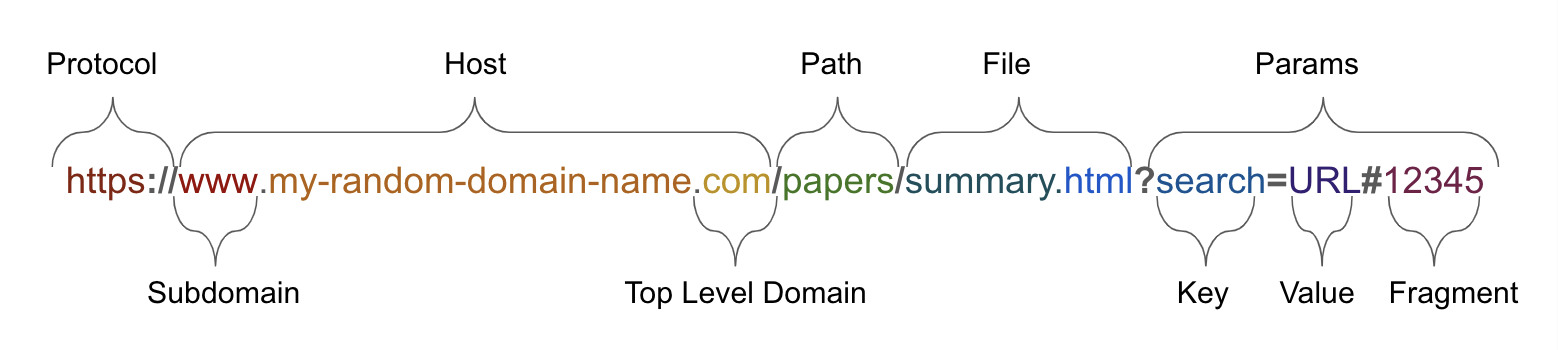
\includegraphics[scale=0.6]{images/URL_parts.png}
}
\caption{Structural components of a URL requiring specific feature engineering treatment}
\label{fig:url_structure}
\end{figure*}

Common approaches to feature engineering on URLs include string patterns and regular 
expressions to identify key sequences and lexical properties 
\cite{Kan2004,Garera2007,Mamun2016,Tupsamudre2019}, 
creation of lookup tables or likelihood scores based on key sequences
\cite{Meshkizadeh2010}, n-gram or bag of words models \cite{Baykan2009,Verma2017}, 
the generation of task specific word embedding vectors based on a segmentation of the 
URL \cite{Le2018,Qiu2020} and the usage of domain name servers or registrars for 
ancillary information about the domain registration 
and server configuration\cite{Canali2011,Li2020}. 
In many modern approaches to malicious URL detection
multiple feature engineering approaches are typically combined\cite{Sayamber2014,Li2020}.
Increasingly, sophisticated methods are used to combine, select or learn from 
combinations of features to adapt to changing requirements, particularly in 
internet security applications\cite{Sountharrajan2020,Li2020}.

Some authors have emphasized that URLs are sequences of characters and require 
feature extraction methods that respect 
this sequential nature\cite{Le2018,Vazhayil2018}. 
They have turned to developing neural network approaches
based on convolutional or recurrent layers for learning these sequential structures.
However, the ordering of key features within URLs is predominantly fixed as shown 
in Figure \ref{fig:url_structure}. The core elements of URL structure occur at 
fixed positions within the sequence, in contrast to human language
sequences which are built from flexible grammars that allow variable positioning of 
most key elements. The inherent structure of URLs has been demonstrated to be a source 
of information that can be exploited in algorithm design \cite{Shih2004}. Furthermore,
there are psychological and social elements to URL construction (such as the use of 
common brand names in subdomains for phishing attack URLs \cite{Tupsamudre2019}), 
which emphasize the utility of feature engineering techniques that
respect the inherent structure of URLs.

Typically, researchers employ feature engineering strategies to exploit these 
potential sources of information
in ways that are appropriate for a given task. However, while there are wide variety
of approaches that are inconsistently applied, there have been limited studies into
the overall effectiveness of different strategies across a range of applications.

In this work we develop a feature engineering library that maintains an ontology of 
URL features related to underlying structure of the URL. In addition we provide a 
method for visualising the importance of features across the URL structure. 
These techniques can prove useful for analysing features for problems that
consist of moving targets and require broad sets of potential features and 
efficient feature selection \cite{Basnet2012}.
We present an open source package for generating features within these
ontologocal classes and apply them to a variety of tasks. We present our results as a
cross-task evaluation of URL features. The strength of our approach lies in the 
ability to both understand how machine learning models use URLs in decision making, 
as opposed to the black-box problem with neural network
models that treat the URL as a text sequence. In addition, the cross-task evaluation 
we perform provides insight into what works within different domains. 
This is critical as many machine learning problems that rely on URLs require
models built on relatively small datasets, so that new patterns of fraud and 
behaviour can be detected rapidly.

\section{Methodology}

The structural components of a URL (as illustrated in Figure \ref{fig:url_structure}) 
are listed in Table \ref{tab:components}.
We include an overview of the information source in each of those components and 
highlight how these components relate to machine learning features.

\begin{table*}
\caption{URL Components and Feature Information}
\label{tab:components}
\resizebox{\columnwidth}{!}{%
\begin{tabular}{|l|l|l|}
\toprule
Component    &Subcomponent      &Type of Feature Information       \\
\midrule
Protocol     &                  &Type of content, technology, security of transmission             \\
\midrule
Domain       &                  &Textual data indicating general purpose      \\
             &Subdomain         &Specific purpose or categorisation of content           \\
             &Top Level Domain  &Business or service purpose, authenticty, geograpahy, age           \\
\midrule
Path         &                  &Content structure, file or operation system, application type or structure         \\
\midrule
File         &                  &Naming of specific content, psychological intent, executable or static types      \\
\midrule
Parameters   &                  &Substructure of content, personalization, security, tracking         \\
             &Keys              &Set of categories used to differentiate substructure        \\
             &Values            &Set of values for substructure, indication of page content        \\
             &Fragment          &Labels for specifc substructure, source of new application customisation        \\
\bottomrule
\end{tabular}
}
\end{table*}

We design a feature extraction library for URLs that generates features specific 
to each component of the URL independently using a naming convention that permits 
separation and grouping for analysis.
Previous work has presented datasets for specific problems where the features
are provided with a similar structural grouping\cite{Vrban2020}. However, we provide 
our feature extraction application designed so that any specific subset of these 
features can be extracted and analysed for a specific task.

We apply this library to multiple machine learning tasks using only URLs as the 
input variable. We choose these tasks such that they span very different classes 
of problems and dataset sizes. We experiment with multiple standard machine 
learning techniques and evaluate the impact of the URL features using the SHAP 
package for feature importance. We develop a process
for analysing these features within the logical structure of the URL.

\subsection{Data}
The data used in this study was colated from a range of sources to represent a variety of
Internet resource classification problems containing URLs as the primary feature.
The ISCX Malicious URL classification dataset contains malware, spam and phishing URLS
that need to be discriminated against a set of benign URLs\cite{Mamun2016}.
The world wide web knowledge base (WebKb) 4 Universities data set contains a wide
range of university URLs categorised into multiple topic categories\cite{Craven1998}.
The Syskill \& Webert webpage ratings dataset containing webepages across 4 categories
with a human generated categorisation for determining personal preferences in webpage
content\cite{Pazzani1996}. Finally, we utilise the Kaggle DMOZ dataset that contains
a large set of topic categorised URLs\cite{dmoz}.

These 6 URL classification problems are summarised in Table \ref{tab:data}, where we
show the number of records, the cardinality of the target classes, and the proportion
of the data that belongs to the most common class in the set.

\begin{table}
\caption{Datasets}
\fontsize{3pt}{3pt}\selectfont
\label{tab:data}
\resizebox{\columnwidth}{!}{%
\begin{tabular}{|l|r|r|r|}
\toprule
Dataset              &Records        &Classes  &Majority    \\
\midrule
spam                 &47,378          &2       &75\%        \\
Malware              &46,944          &2       &75\%        \\
Phishing             &45,343          &2       &78\%        \\
WebKb 4Uni           &8,284           &7       &45\%        \\
Syskill \& Webert    &330             &3       &68\%        \\
DMOZ                 &1,562,978       &15      &16\%        \\
\bottomrule
\end{tabular}
}
\end{table}

We generate all URL features for each of these datasets and then apply a range of 
machine learning
techniques to build classifiers that can be analysed for key features on each task.

\begin{table*}
\caption{URL Features}
\label{tab:features}
\resizebox{\columnwidth}{!}{%
\begin{tabular}{|l|l|l|l|}
\toprule
Group         &Feature              &Type        &Definition  \\
\midrule
Protocol      &protocol\_name         &Category    &The exact internet protocol name    \\
              &protocol\_type         &Category    &Internet protocol categorised by its purpose    \\
              &protocol\_exists       &Boolean     &Flag indicating presence or absence of internet protocol   \\
\midrule
Host          &host\_is\_ip           &Boolean     &Flag indicating if the host is an IP address    \\
              &host\_has\_port        &Boolean     &Flag indicating if a port number is explicitly specified    \\
              &domain\_len            &Numeric     &Character length of the domain name (minus TLD and subdomain)     \\
              &domain\_alpha          &Numeric     &Proportion of characters in the domain that are letters    \\
              &domain\_sections       &Numeric     &Count of period separated domain sections    \\
              &subdomain              &Category    &The text value of the subdomain  \\
              &subdomain\_type        &Category    &Categorisation of the purpose of the subdomain \\
              &subdomain\_freq        &Numeric     &Frequency of the subdomain in internet traffics    \\
              &tld\_name              &Category    &Top Level Domain Name    \\
              &tld\_type              &Category    &Top Level Domain extension categorised by purpose    \\
              &tld\_freq              &Numeric     &Top Level Domain extension frequency in internet traffic   \\
\midrule
Path          &path\_depth            &Numeric     &The depth of the directory path between host and file   \\
              &path\_1st\_wd          &Category    &The first distinct word in the path longer than 2 chars  \\
              &path\_1st\_wd\_prefix  &Category    &The first 3 chars of the first distinct word in the path > 2 chars   \\
              &path\_wd\_count        &Numeric     &Count of distinct words in the path between host and file   \\
              &path\_wd\_len          &Numeric     &The mean length of the individual words in the path  \\
              &path\_has\_date        &Boolean     &Flag indicating if a date is detected in the path  \\
              &path\_is\_home         &Boolean     &Flag indicating if the path starts with a home directory    \\
\midrule 
File          &file\_len              &Numeric     &The character length of the target file    \\
              &file\_1st\_wd          &Category    &The first distinct word in the file name  \\
              &file\_1st\_wd\_prefix  &Category    &The first 3 chars of the first distinct word in the filename  \\
              &file\_wd\_count        &Numeric     &The count of words longer than 2 chars in the file name   \\
              &file\_wd\_len          &Numeric     &The mean length of the individual words in the file name  \\
              &file\_ext              &Category    &The exact file extension e.g. "exe" or "php"    \\
              &file\_type             &Category    &File extension categorised by function \& purpose (e.g. Static or dynamic)   \\
              &file\_ext\_exists      &Boolean     &Flag indicating presence of a file extension for the URL target  \\
\midrule
Params        &params\_len            &Numeric     &The character length of the parameter string    \\
              &params\_count          &Numeric     &The count of the key value pairs in the param string    \\
              &params\_match          &Boolean     &Flag indicating if the count of keys and values in the param string match    \\
              &params\_has\_url       &Boolean     &Flag indicating presence of a raw URL within the parameter string   \\
              &params\_enc\_url       &Boolean     &Flag indicating presence of an encoded URL within the parameter string   \\
              &params\_enc\_char      &Boolean     &Flag indicating presence of an encoded character within the parameter string   \\
              &params\_frag\_len      &Numeric     &Length of a hash delineated fragement at the end of the parameter string   \\
              &keys\_count            &Numeric     &Count of the distinct keys used in the parameter string  \\
              &keys\_len              &Numeric     &The mean length of the individual keys in the params  \\
              &keys\_numeric          &Numeric     &The proportion of numeric characters in the param keys \\
              &values\_count          &Numeric     &Count of the distinct values used in the parameter string  \\
              &values\_len            &Numeric     &The mean length of the individual values in the params  \\
              &values\_numeric        &Numeric     &The proportion of numeric characters in the param values \\
              &frag\_len              &Numeric     &The character length of the fragment string    \\
              &frag\_secs             &Numeric     &Count of distinct sections in the fragment string delimited by [?\&=]  \\
              &frag\_enc\_char        &Boolean     &Flag indicating presence of an encoded character within the fragment string    \\
\bottomrule
\end{tabular}
}
\end{table*}

\subsection{Feature Generation}

We generate URL features using a set of functions that focus on distinct types of 
features applied to specific regions across the URL. 
This permits users to apply subsets of functions that define only the features they
require. In addition we create a group of global features that contain general string 
properties of the entire URL, rather than specific regions. 
The complete set of features, along with their categorisation and definition
are outlined in Table \ref{tab:features}.

These URL feature functions are available in our open source implmentation and 
python package \emph{url2features}. 
The package is designed such that it can process large files in chunks and will 
only add the specific sub-groups of
features a user requests. In addition, the naming convention is designed so that 
features relating to specific
regions of the URL can be identified and analysed as a group.

\begin{lstlisting}[language=Bash,label={code:cli}, caption=Install and invoke the url2features package from CLI]
pip install url2features
url2features -columns=URLCOL -host -tld input.csv > output.csv
\end{lstlisting}

The commands for installing and invoking the \emph{url2features} package from the 
command line are shown in Listing \ref{code:cli}. 
When executing this code it will take the tabular data inside the file 
\emph{input.csv} and then apply feature 
engineering on the column named \emph{URLCOL}. 
The features to be created are defined by the switches 
$-host$ and $-tld$ for the host and top level domain features. 
By default the application outputs to
STDOUT, so in this example we are redirecting the output of the program to 
create a new file \emph{output.csv}. 

\begin{lstlisting}[language=Python,label={code:skl}, caption=Usage of url2features with scikit-learn pipelines ]
from url2features.pipeline import URLTransform
from sklearn.linear_model import SGDClassifier
from sklearn.pipeline import Pipeline

pipeline = Pipeline([
    ('urltransform', URLTransform(['URLCOL'],['host','tld']) ),
    ('clf', SGDClassifier(loss='log') ),
])
\end{lstlisting}

The package can also be invoked programmatically and included inside a machine 
learning framework like 
scikit-learn pipelines\cite{pedregosa2011scikit}. 
This is shown in Listing \ref{code:skl}, where the
same two feature engineering functions (host and tld) are included 
as feature transformers in a machine learning pipeline. 
The advantage of this approach is that these transformations can be built into a single
serialised model for deployment.

\subsection{Feature Importance}

We use the SHAP\cite{Lundberg2017} package to calculate feature importance using a 
small holdout test set of 80-100 samples per experiment. 
We aggregate the Shapley values for these sample points to calculate the mean
absolute contribution of each feature, as is typically done in Shapley feature 
importance plots.

For our URL feature analysis, we then group these individual feature importance 
values by the specific URL segment that the feature was derived from, 
using Figure \ref{fig:url_structure} as a guide to these segments. 
We sum the feature importance for all features within a URL segment to allow us to plot the
segment contributions to model performance. We provide a thin grey coloured line 
covering the entire segment
which captures the importance of global features (like URL length). 
If the script is applied to a dataset with
more than just URL features then all non-URL fetaures would be grouped into this global group. All segment specific
URL features are plotted below their segment in a canonical example URL.

These plots allow for a structural understanding of how URL data
contributes to predictive performance of a model and permits the comparison of 
feature importance 
across the six problems in this study. 
The script for generating these plots is provided as part 
of the source code for the `url2features` package.

\section{Results}

A set of standard machine learning pipelines are applied to each of the six 
problems. Each approach is applied using default parameters, without any fine tuning. 
We use feature preprocessing modules appropriate for each class
of model. All details are available in the source repository for the experiments. 
The performance of the models is shown in Table \ref{tab:results}, where we show 
Balanced Accuracy of each model on the holdout data, as this
metric is appropriate and comparable across all six problems. 

\begin{table}
\caption{Machine Learning Results}
\fontsize{3pt}{3pt}\selectfont
\label{tab:results}
\resizebox{\columnwidth}{!}{%
\begin{tabular}{|l|r|r|r|r|}
\toprule
Dataset              &NB     &LR    &XT    &LGBM     \\
\midrule
Spam                 &1.00   &1.00  &1.00  &1.00     \\
Malware              &0.65   &0.93  &0.99  &1.00     \\
Phishing             &0.89   &0.98  &0.99  &1.00     \\
WebKb 4Uni           &0.30   &0.36  &0.58  &0.49     \\
Syskill \& Webert    &0.39   &0.35  &0.37  &0.33     \\
DMOZ                 &0.12   &0.17  &0.29  &0.25     \\
\bottomrule
\end{tabular}
}
\end{table}

\begin{figure*}
\centering
\resizebox{\columnwidth}{!}{%
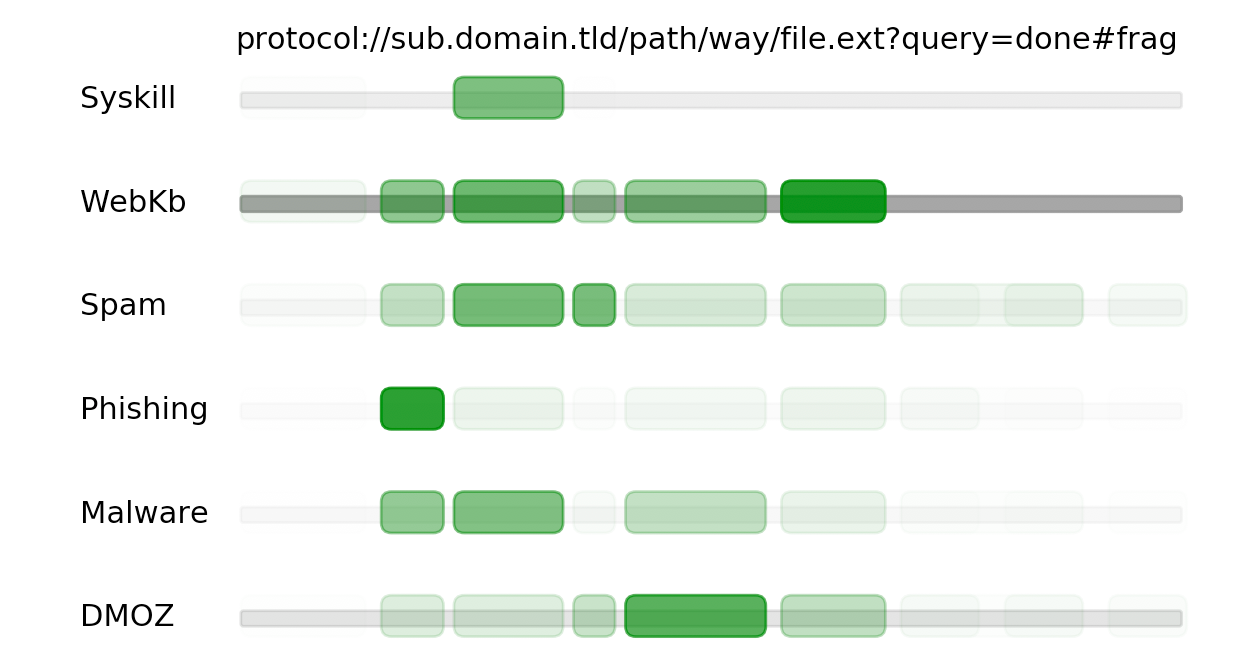
\includegraphics[scale=0.8]{images/URL_importance.png}
}
\caption{Structural Depiction of URL Feature Importance}
\label{fig:importance}
\end{figure*}

The table of results indicates that internet security problems appear much more 
amenable to URL based classification. All three of these problems result in high 
performing classifiers. By comparison the topic and user preference classification
tasks achieve far more modest performance. It is worth noting that these problems 
are hindered by both higher cardinality in the classification targets and greater 
variability in dataset size, 2 of the 3 data sets are much smaller than any of the 
security datasets. However, the performance on the very large DMOZ
dataset strongly suggests that, in general, URL based topic classification is 
likely to remain a difficult problem. 

We used the results from the best performing classification model for each 
individual problem and generated the SHAP values for the records in the test dataset. 
These records are then used to generate the URL Structure Feature Importance Plot 
shown in Figure \ref{fig:importance}. This plot aggregates the importance of individual
features into their region of origin within the URL structure. 
Allowing us to visualise the source of signal for
each task and compare features across tasks.

We see that there is substantial variability across all classification tasks in 
these experiments.
The protocol and parameters sections remain mostly devoid of signal, with the 
exception of the Spam URL classification task, where we see value in the URL 
parameter features. The domain, path and file regions are the predominant sources
of signal across these tasks. Nevertheless, the emphasis changes between them. 
The subdomain appears particularly
important for the phishing URL identfication, whereas the URL from domain to filename 
is important for the WebKb classification data.

The internet security problems appear to derive less utility from the global 
features when compared to the three topic classification problems, as is 
indicated by the strength of the grey lines through the middle of the plot 
for each task. This suggests that these problems rely more heavily on the 
information from specific components of the URL structure.

The contributions of the domain remain high across all problems evaluated. 
However, whether the key elements is the
domain name itself, the subdomain or the top level domain varies considerably 
across the tasks and does not appear consistant across the top broad categories 
of security and topic classification problems. 
This suggests that data scientists and machine learning engineers
need to test these features on a task by task basis rather than relying on heuristics.


\section{Conclusion}

We have described the structural elements of a URL from which context specific 
features can be extracted.
These features tend to be used indepedently within different problem types and 
tuned for specific purposes. 
In this paper we have described an open source URL feature generation package 
that is both sensitive to the 
source of information within each component and sufficiently flexible for general use. 
We conducted experiments
using the features across a range of indepenent URL classification tasks. 

Our experiments demonstrated that the various structural regions play different 
roles across these tasks, exhibiting varying levels of importance. 
Some patterns (like the strength of global URL features)
could be attributed to broader categories of the task, while others appear task specific.
We have observed that the domain name, with its subcomponents, is a strong and 
consistent contributor to the performance of models across tasks. The source of 
information from within the domain varies, but it remains
a rich source of information for machine learning tasks that rely on the URL as a 
central feature.


\bibliographystyle{ieeetr}
\bibliography{refs}

\end{document}
\endinput
